\section{Architecture technique cible}
\label{sec:technique}

\subsection{Principes techniques}
L'architecture technique (figure~\ref{fig:technique}) découle des principes de souveraineté, de sécurité et d'interopérabilité. Elle repose sur un hébergement dans un cloud souverain conforme aux exigences de la DGSSI, sur une segmentation en zones étanches, sur des composants conteneurisés orchestrés par Kubernetes, et sur un bus d'événements qui découple les applications. Les sites physiques (CEDI, centres de production) restent connectés par le réseau interministériel sécurisé.

\begin{figure*}[t]
\centering
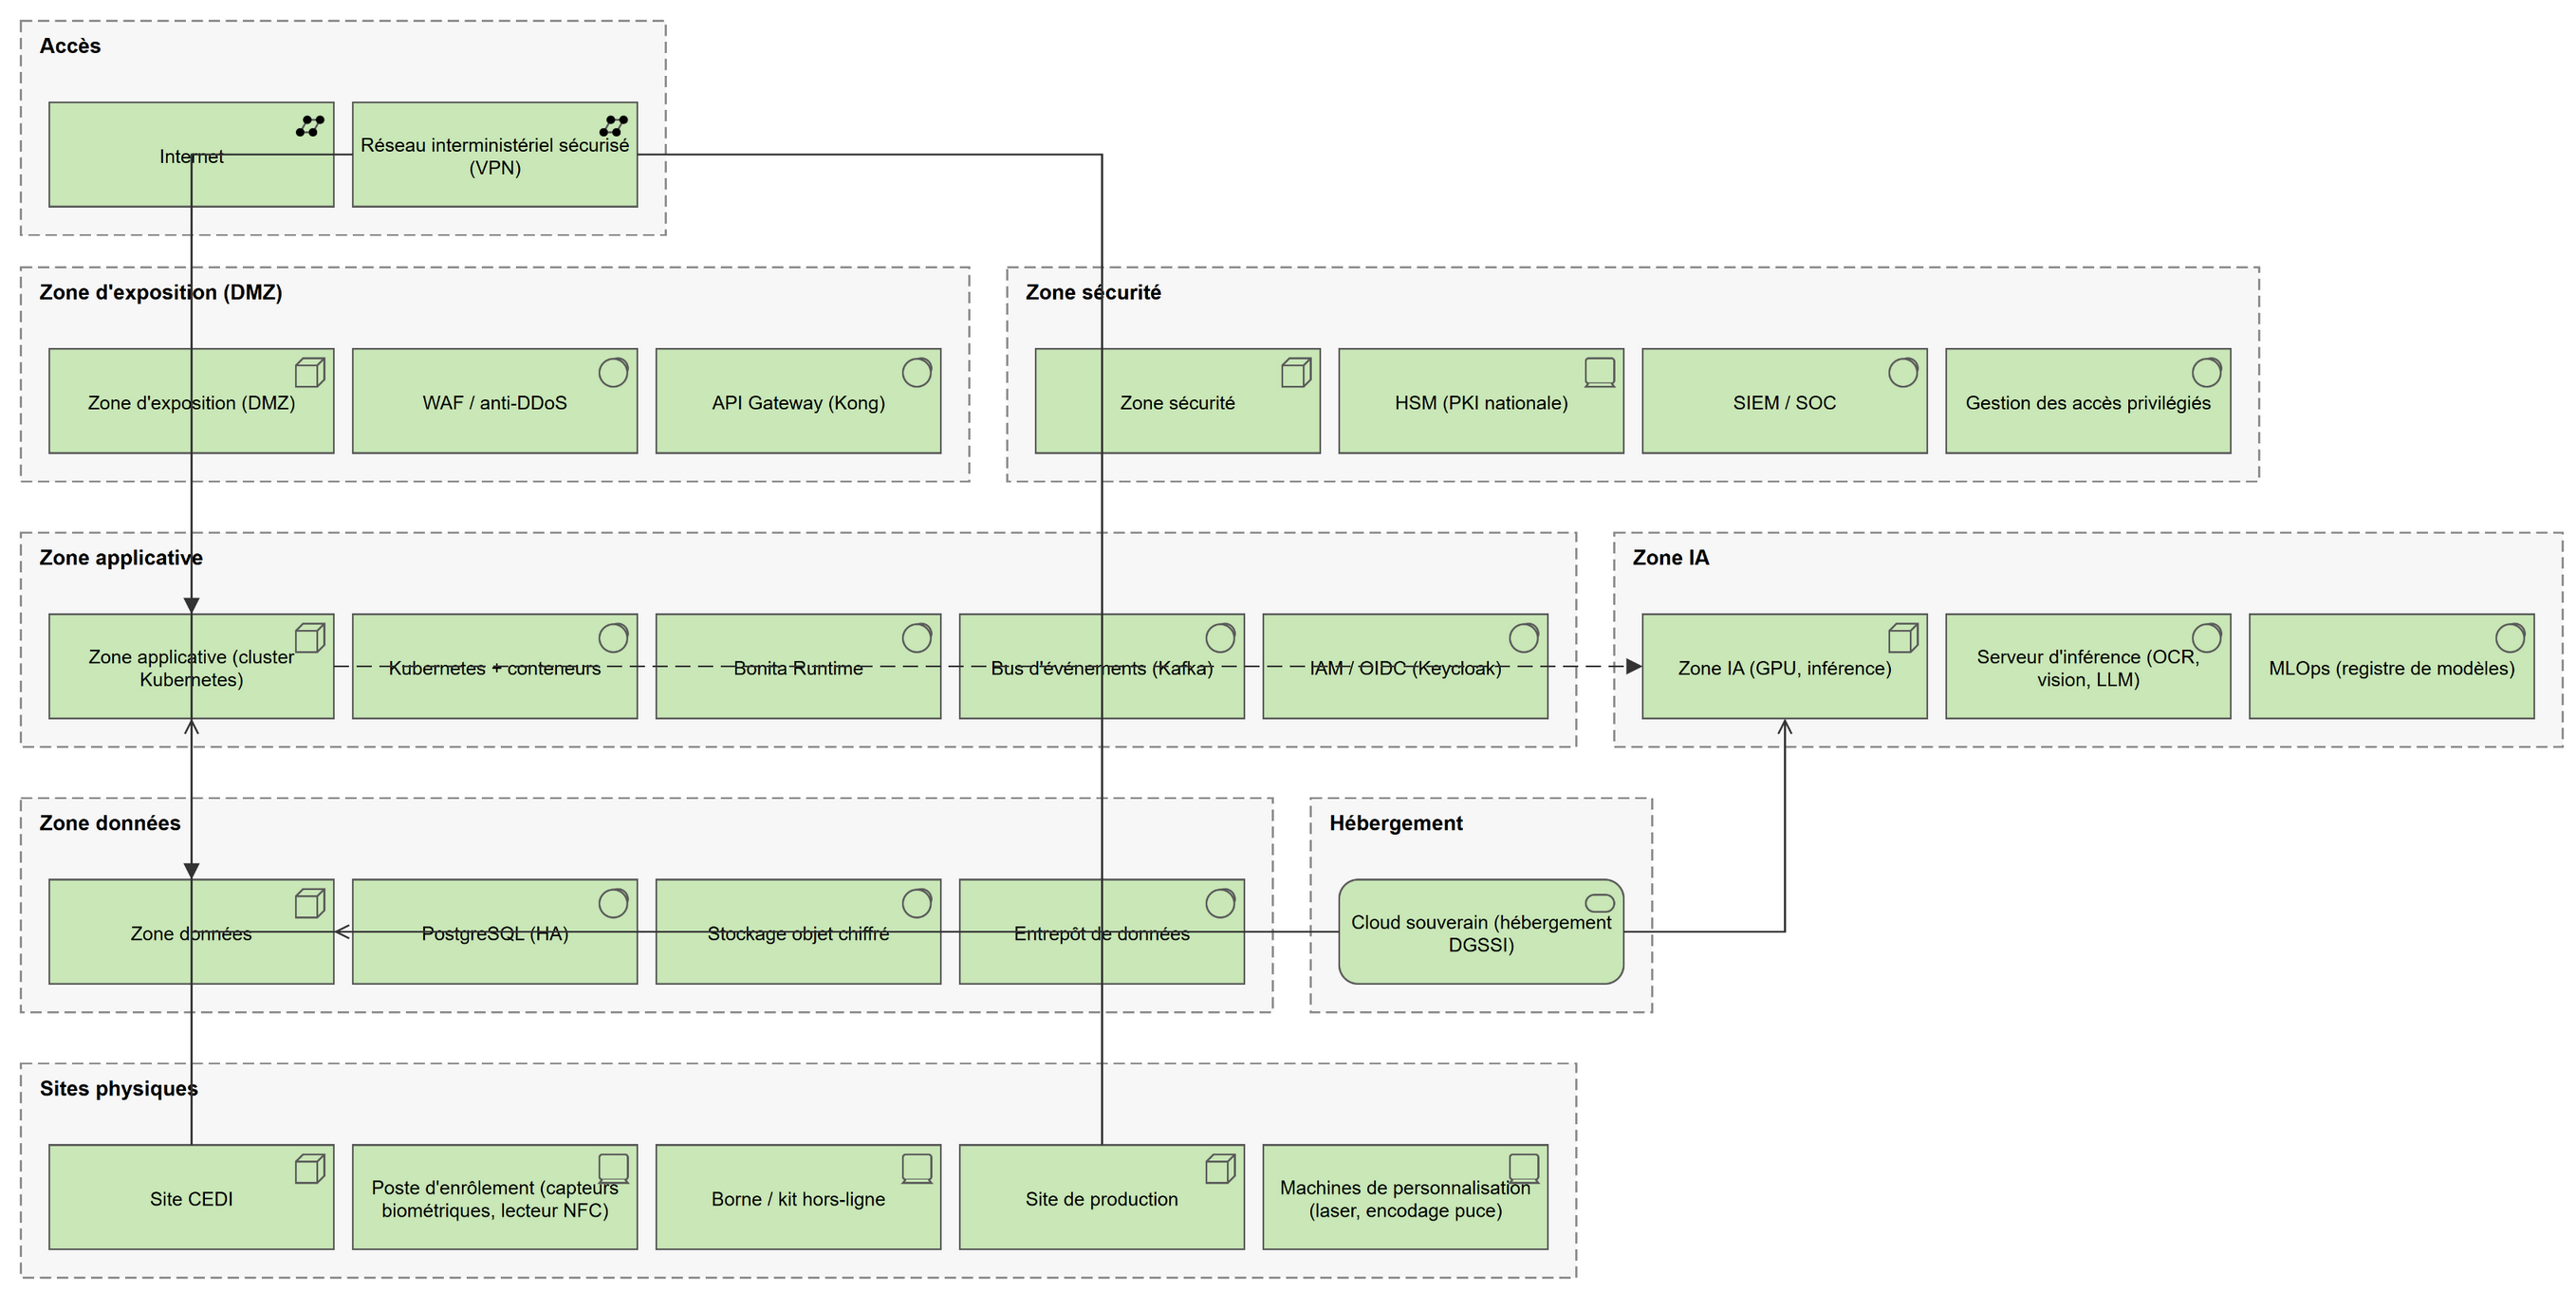
\includegraphics[width=0.98\textwidth]{archimate/V5_technique.png}
\caption{Architecture technique cible~: zones d'exposition, de sécurité, applicative, d'IA et de données~; sites physiques.}
\label{fig:technique}
\end{figure*}

\subsection{Zones}
\paragraph{Zone d'exposition} Un pare-feu applicatif et une protection contre le déni de service filtrent les accès depuis Internet. La passerelle d'API (APP-11) y est exposée~; elle applique l'authentification des clients, les quotas et la journalisation. Les canaux citoyens (portail, application mobile) ne dialoguent qu'avec cette passerelle.
\paragraph{Zone applicative} Le cluster Kubernetes héberge le moteur Bonita, les services métier et le bus d'événements. Le serveur d'identité (OpenID Connect) fédère les authentifications internes et délègue celles des citoyens à la plateforme Tiers de Confiance, qui reste un système distinct, conformément à son modèle sans registre central \cite{dgsn2023tcn}.
\paragraph{Zone de données} Les bases relationnelles en haute disponibilité portent les demandes et les rendez-vous~; un stockage objet chiffré conserve les pièces téléversées avec une durée de rétention limitée~; l'entrepôt de données alimente la BI à partir de données pseudonymisées.
\paragraph{Zone d'IA} Un serveur d'inférence dédié, doté d'accélérateurs graphiques, exécute les modèles de reconnaissance de caractères, de vision, de prévision et le modèle de langue de l'assistant. Le registre de modèles et la chaîne MLOps assurent le versionnement, les tests de non-régression et la surveillance de la dérive. Aucun flux de cette zone ne sort du territoire.
\paragraph{Zone de sécurité} Les modules matériels de sécurité (HSM) protègent les clés de la PKI nationale utilisées pour la personnalisation des puces et la signature des récépissés~; un SIEM centralise les journaux et alimente le centre opérationnel de sécurité~; la gestion des accès privilégiés encadre les administrateurs.
\paragraph{Sites physiques} Les postes d'enrôlement des CEDI (capteurs biométriques, lecteur NFC, scanner de QR code) et les kits hors-ligne fonctionnent en mode dégradé en cas de coupure réseau et se resynchronisent ensuite. Les centres de production conservent leurs machines de personnalisation, intégrées par le bus d'événements pour la remontée des statuts.

\subsection{Sécurité et conformité}
Le tableau~\ref{tab:secu} résume les mesures de sécurité associées aux principaux risques. Les niveaux d'assurance d'identité et d'authentification s'inspirent des catégories définies par les référentiels internationaux \cite{nist80063}~: l'accès à une demande en cours requiert une authentification forte via l'identité numérique, et la remise à domicile exige une vérification biométrique du porteur.

\begin{table}[h]
\caption{Risques et mesures de sécurité}
\label{tab:secu}
\centering
\small
\begin{tabularx}{\columnwidth}{lX}
\toprule
\textbf{Risque} & \textbf{Mesure} \\
\midrule
Usurpation d'identité en ligne & Authentification forte OpenID Connect via la plateforme Tiers de Confiance, détection du vivant à l'enrôlement \\
Fuite de pièces justificatives & Chiffrement au repos et en transit, rétention limitée, accès journalisés, séparation des zones \\
Fraude documentaire & Contrôle automatique des pièces, rapprochement avec l'état civil, instruction humaine des cas douteux \\
Compromission des clés & HSM certifiés, double contrôle des opérations, rotation des clés \\
Biais ou dérive des modèles & Évaluation d'équité avant mise en service, surveillance continue, décision humaine sur toute alerte \\
Indisponibilité & Haute disponibilité multi-zones, mode dégradé des CEDI, plan de reprise \\
Non-conformité CNDP & Registre des traitements, consentement explicite, minimisation, analyse d'impact \\
\bottomrule
\end{tabularx}
\end{table}

\subsection{Dimensionnement}
Avec près de 3,7 millions de cartes produites en 2025 \cite{lavieeco2025bilan}, le système doit absorber en moyenne 15\,000 demandes par jour ouvré et des pointes trois fois supérieures lors des campagnes de renouvellement. Le contrôle documentaire, à raison de trois pièces par demande et d'un temps d'inférence de l'ordre de la seconde, mobilise quelques accélérateurs graphiques seulement~; la prévision d'affluence s'exécute en lot quotidien. Le dimensionnement critique porte sur le stockage des pièces (plusieurs téraoctets par an avant purge) et sur la capacité biométrique du référentiel, déjà en place.
